%*****************************************
\chapter{Grundlagen}\label{ch:preliminaries}
%*****************************************

\section{Medizinische Informatik}

\subsection{Informationssysteme im Gesundheitswesen}

\begin{definition}[System]
\enquote{Ein System ist eine Menge an Elementen und deren Beziehungen.}
(Aus dem Englischen von \citet[S.~30]{bb})
\end{definition}
\begin{definition}[Informationssystem]
\enquote{Ein Informationssystem ist ein System das Daten, Informationen und Wissen speichert und verarbeitet.}
(Aus dem Englischen von \citet[S.~30]{bb})
\end{definition}

\begin{definition}[Informationssystem im Gesundheitswesen]
\enquote{Ein Krankenhausinformationssystem ist das sozioökonomische Subsystem eines Krankenhauses, welches die gesamte Informationsverarbeitung sowie die zugehörigen menschlichen Akteure in deren respektiven Informationsverarbeitungsrollen umfasst.}
(Aus dem Englischen von \citet[S.~37]{bb})
\end{definition}

\subsection{Daten, Informationen, Wissen}
Daten sind die physische Repräsentation von Informationen oder Wissen, also zum Beispiel die Zeichenkette \enquote{Universitätsklinikum}.
Daten können neu interpretiert werden.
Informationen hingegen sind Fakten, die gegebenenfalls aus Daten hervorgehen, also zum Beispiel die Information, dass Frau Mustermann verantwortlich für das jährliche IT-Budget des Uniklinikum Leipzigs ist.
Wissen ist eine generelle Information über einen Begriff \citep[S.~29]{bb}, also zum Beispiel, dass die Leiterin des Informationsmanagements für das jährliche IT-Budget ihrer Einrichtung verantwortlich ist.
Es gibt auch andere Definitionen dieser drei Begriffe, hier werden allerdings diese verwendet.

\section{Geschriebene Sprache}

In der Schriftsprache werden Daten, Information und Wissen durch Sätze überbracht.
Dies ist ein sehr komplexes Thema, hier werden allerdings nur die für diese Arbeit wichtigen Begriffe betrachtet.

\subsection{Wort, Begriff und Konzept}

Ein \emph{Wort} ist eine Anreihung von Lauten, die zusammengesetzt eine Bedeutung haben.
Ein \emph{Begriff} ist ein Wort, welches ein Objekt, eine Person o.ä. beschreibt.
Es kann mit dem englischen Wort \enquote{concept} übersetzt werden.
Ein \emph{Konzept} (Englisch: \enquote{draft}) ist eine abstrakte Idee oder ein konkreter Plan.
Begriffe erklären also existierende Dinge bzw. Gegenstände oder Gedanken, Konzepte hingegen Vorhaben oder oder Schemen.
\todo{Beispiel aus SNIK}
\todo{Duden zitieren}

\subsection{Synonyme, Homonyme und Ambiguität}

Synonyme existieren, wenn zwei verschiedene Wörter auf den gleichen Begriff verweisen, z.B. \enquote{}.
Homonyme meinen, dass ein Wort zwei verschiedene Begriffe beschreibt, also z.B. die Bank, welche entweder ein Geldinstitut oder eine Parkbank sein kann.

\todo{evtl. Beispiel aus SNIK}
Ambiguität oder Mehrdeutigkeit bedeutet, dass ein Satz oder eine Wortgruppe verschieden interpretiert werden kann.
Zur Auflösung dieser Unklarheit wird meistens mehr Kontext benötigt.
Homonymität kann also auch als Ambiguität eines einzelnen Wortes beschrieben werden.
\todo{Beispiel aus SNIK}

\subsection{Lexik, Syntax und Semantik}

Die \emph{Lexik} beschreibt die Wortarten.
Es wird zwischen flektierbaren und unflektierbaren Wortarten unterschieden.
Verben, Substantive, Adjektive, Artikel und Pronomen kann man konjugieren bzw. deklinieren.
Sie werden auch flektierbar genannt.
Die Form unflektierbarer Wortarten ist unveränderlich, sie enthalten Partikel wie Adverbien und Interjektionen \citep[S.~505]{deutschbuch}.
Die \emph{Syntax} behandelt den Satzbau und somit die Satzglieder wie Subjekt, Prädikat und Objekt oder Satzarten wie der Aussage-, Aufforderungs- und Fragesatz und deren Unterarten.
Unterarten von Fragesätzen sind  die Entscheidungsfrage, wo ein Wahrheitswert als Antwort erwartet wird, die Ergänzungsfrage, wo nach Informationen gesucht wird, und die rhetorische Frage, auf welche keine Antwort erwartet wird.
Besonders Ergänzungsfragen, welche typischerweise mit einem Fragewort beginnnen, sind in dieser Arbeit wichtig.
Die \emph{Semantik} beschäftigt sich mit der Bedeutung der einzelnen Wörter und fokussiert sich dabei besonders, aber nicht nur, auf Präpositionen, Adjektive und Adverben.
Sie beschäftigt sich demnach auch mit Synonymen und Homonymen, es wird z.B. versucht, alle möglichen Bedeutungen eines Wortes zu erfahren.
\todo{Beispiele aus SNIK}

\section{Semantic Web}

\subsection{URIs, IRIs und URLs}
\ac{uri} werden zur eindeutigen Zuordnung von Zeichenketten zu beliebigen Ressourcen verwendet \citep{uri}.
\ac{url} ist eine URL mit konkreten Zugriffsmöglichkeiten auf die Ressource \citep{url}.
Ein \ac{iri} ist ein URI mit einer größeren Anzahl an möglichen Zeichen, da es auch nichtlateinische Schriftzeichen erlaubt.

\subsection{World Wide Web}
Das \ac{www} wurde 1991 von Tim Berners-Lee entwickelt.
Es ermöglicht freien Zugriff auf und Austausch von Daten über das \ac{http}.
Die Standards zu dieser Kommunikation setzt das \ac{w3c}, dessen Direktor Berners-Lee ist.
Das Format der Dokumente wird durch die \ac{html} beschrieben, welche ebenfalls vom \ac{w3c} kontrolliert wird \citep{www}.

\subsection{Semantic Web}
Im Gegensatz zu \ac{www}, einem Web der Dokumente, ist das Semantic Web ein Web der Daten.
Es ist außerdem nicht nur ein verwendbares Artefakt wie das \ac{www}, sondern auch ein Forschungsfeld \citep{semanticwebreview}, das sehr stark von anderen Forschungsfeldern, wie etwa Deep Learning und künstlicher Intelligenz, abhängig ist. Teile des Forschungsfeldes sind Ontologien, Linked Data und sogenannte Knowledge Graphs, auf die hier aber nicht weiter eingegangen werden wird.
Das Semantic Web als nutzbares Objekt besteht aus strukturierten Daten, sodass man, im Gegensatz zum \ac{www}, Informationen direkt abfragen kann und nicht erst die HTML-Dokumente auswerten muss.
\daurl{bb}{http://www.snik.eu/ontology/bb/}
\daurl{ciox}{http://www.snik.eu/ontology/ciox/}
\daurl{ex}{http://www.example.org/}
\subsection{RDF}
\begin{table}[h]\centering\scriptsize
  \begin{tabulary}{\textwidth}{rrl}
    \toprule
    Funktion & Beispiel 1 & Beispiel 2 \\
    \midrule
    Subjekt & \aurl{bb}{ChiefInformationOfficer} & \aurl{ex}{ErikaMustermann} \\
    Prädikat & \aurl{meta}{isResponsibleForEntityType} & \aurl{rdf}{type} \\
    Objekt & \aurl{bb}{AnnualITBudget} & \aurl{ciox}{ChiefInformationOfficer} \\
    \bottomrule
  \end{tabulary}
  \caption{Beispiele für RDF-Tripel}
  \label{tab:rdftripleexample}
\end{table}

Das \ac{rdf} ist das grundlegende zur Beschreibung des Semantic Webs genutzte Format \citep[S.~35]{semanticwebgrundlagen}.
Mithilfe dieser formalen Sprache, die erstmals 1999 durch das \ac{w3c} spezifiziert wurde, sollten zuerst Metadaten modelliert werden.
Aufgrund dem Fokus auf der Weiterverarbeitbarkeit der Daten ist es für seine Nutzer gut zur Modellierung des Semantic Webs geeignet.
RDF wird in Tripeln aus Subjekt, Objekt und Prädikat modelliert.
Es verhält sich hierbei wie in einem einfachen deutschen Satz, das Prädikat beschreibt also die Beziehung zwischen dem Subjekt und Objekt.
Alle drei werden normalerweise als \acp{uri} angegeben \citep{linkeddatadesignissues}.
Beispiel für solche Tripel aus \acp{uri} sind in \cref{tab:rdftripleexample} zu sehen:
Die Leiterin des Informationsmanagements (Subjekt) verantwortet (Prädikat) das jährliche IT-Budget (Objekt).
Beim zweiten Beispiel ist wichtig, dass \aurl{bb}{ChiefInformationOfficer} und \aurl{ciox}{ChiefInformationOfficer} nicht auf das gleiche Wissen zeigen.
Durch den \emph{Prefix} wird die genaue und einzigartige Adresse festgelegt.
Die Wahl des Präfixes ist hierbei den Verantwortlichen überlassen, wichtig ist nur, sie auf eine \ac{http}-Adresse verweisen zu lassen.
Der Präfix \enquote{ex:} wird z.B. häufig für Beispiele benutzt.
Alle in dieser Arbeit verwendeten Präfixe sind in \cref{tab:prefixes} mit ihren \acp{uri} aufgelistet.

\begin{table}[h]\centering
  \begin{tabulary}{\textwidth}{rl}
    \toprule
    Präfix & \ac{uri} \\
    \midrule
    bb & \url{http://snik.eu/ontology/bb/} \\
    coix & \url{http://snik.eu/ontology/coix/} \\
    he & \url{http://snik.eu/ontology/he/} \\
    ob & \url{http://snik.eu/ontology/ob/} \\
    meta & \url{http://snik.eu/ontology/meta/} \\
    rdf & \url{http://www.w3.org/1999/02/22-rdf-syntax-ns\#} \\
    rdfs & \url{http://www.w3.org/2000/01/rdf-schema\#} \\
    ex & \url{http://example.org/} \\
    \bottomrule
  \end{tabulary}
  \caption{In dieser Arbeit verwendete Präfixe}
  \label{tab:prefixes}
\end{table}

\subsection{Ontologien}
\label{sub:ontology}
\enquote{Im Kontext der Informatik ist eine Ontologie eine Menge von repräsentativen Primitiven, welche einen Bereich des Wissens oder eines Diskurses modellieren.
Die repräsentativen Primitiven sind typischerweise Klassen (oder Mengen), Attribute (oder Eigenschaften), und Zusammenhänge (oder Beziehungen zwischen Klassenelementen).
Die Definitionen der repräsentativen Primitiven enthalten Informationen über ihre Bedeutung und Beschränkungen ihrer logisch konsistenten Anwendung.
Im Kontext von Datenbanksystemen kann eine Ontologie als ein Level der Abstraktion von Datenmodellen, analog zu hierarchischen und relationalen Modellen,
gesehen werden, aber dazu gedacht, Wissen über Individuen, deren Attribute, und deren Beziehungen zu anderen Individuen zu modellieren.
Ontologien sind typischerweise in Sprachen, die Abstraktionen weg von Datenstrukturen und Implementationsstrategien ermöglichen spezifiziert;
In Praxis sind die Sprachen von Ontologien in der expressiven Kraft näher an Logik erster Ordnung als alle anderen zur Modellierung von Datenbanken genutzten Sprachen.
Deshalb werden Ontologien als auf dem \enquote{semantischen} Level stehend angesehen, wohingegen andere Datenbankschemen auf dem \enquote{logischen} oder \enquote{physischen} Level sind.
Durch ihre Unabhängigkeit von Datenmodellen niedrigeren Levels werden Ontologien zum Integrieren von heterogenen Datenbanken genutzt,
was die Benutzbarkeit über verschiedene Systeme erlaubt, und die Spezifizierung von unabhängigen, wissensbasierten  Dienstleistungen ermöglicht.
Im Technologie-Stack der Semantic Web Standards sind Ontologien ihre eigene Schicht.
Es gibt nun standardisierte Sprachen und eine Vielzahl an kommerziellen und Open-Source Werkzeugen, um Ontologien zu erstellen und mit ihnen zu arbeiten.
}\\
\textcolor{darkgray}{Aus dem Englischen von \citet{ontologygruber}}

\subsection{Taxonomie}

Nur Beziehungen Subklassen->Klassen \todo{Taxonomie}

\subsection{Individuen und Klassen}
\label{sec:individuenundklassen}
Die Beziehung zwischen Individuum und Klasse entspricht einer Elementbeziehung im Sinne der Mengentheorie der Mathematik, für ein Individuum $e$ einer Klasse $K$ gilt also $e \in K$.
Aus dem Beispiel aus \cref{tab:rdftripleexample} ist also Frau Musterfrau ein Element der Klasse Leiterin des Informationsmanagements.
Dahingegen ist die Beziehung zwischen Unterklassen $U$ und Oberklassen $O$ eine Teilmengenbeziehung ($U \subseteq O$), das heißt, dass jedes Element der Unterklasse auch ein Element der Oberklasse ist.
Echte Teilmengenbeziehungen ($U \subset O$) existieren, wenn jedes Element von $U$ ein Element von $O$ ist, $O$ aber zumindest ein Element enthält, das nicht in $U$ ist \citep[S.~261]{semanticwebgrundlagen}.

\subsubsection{Relationen}
Beziehungen zwischen Individuen untereinander werden \emph{Relationen} genannt.
Relationen können als Teilmenge zwischen Individuen $a \in A$ und $b \in B$ vom kartesischen Produkt der Klassen $A$ und $B$ bezeichnet werden, also gilt $(a,b) \in R$, wenn $R \subset A \times B$ ist.
\todo{über den gesamten Absatz nochmal drüberschauen}
Als Kurzform kann auch $aRb$ geschrieben werden \citep[S.~263]{semanticwebgrundlagen}.
Es gibt nicht nur \emph{binäre} Relationen, also Relationen zweier Elemente, hier werden aber nur diese benötigt.

In \ac{rdf} sind nämlich alle Relationen zweistellig, also Paare.
Die Beschreibung dieser Relation wird \enquote{Property}, also Attribut oder Eigenschaft, genannt.
Properties nehmen die Rolle von Prädikaten an, so ist zum Beispiel \aurl{meta}{isResponsibleForEntityType} ein Property von \aurl{bb}{ChiefInformationOfficer} mit dem Wert \aurl{bb}{AnnualITBudget}.
Sie können auch eingeschränkt werden, indem man ihnen mit \ac{rdf} ihren \emph{Definitionsbereich} mit und \emph{Wertebereich} verändert.
Damit lässt sich einstellen, welche Datentypen als Subjekt und Objekt akzeptiert werden \citep[S.~76]{semanticwebgrundlagen}.
Der Definitionsbereich wird über \aurl{rdfs}{domain} und der Wertebereich über \aurl{rdfs}{range} bearbeitet.

\emph{Literale}, oder auch \emph{Data}-Properties, erfüllen die Funktion der Datentypen.
Sie sind reservierte \acp{uri}, welche die Art des vorhandenen Werts anzeigen.

Properties mit Klassen als Definitions- und Wertebereich werden auch \emph{Object}-Properties genannt.
So ist in \cref{tab:rdftripleexample} \aurl{bb}{isResponsibleForEntityType} ein Property mit \aurl{meta}{Role} als Definitions- und \aurl{meta}{EntityType} als Wertebereich,
sie sind also Eigenschaften von Objekten.

\subsubsection{Wissensbasen}
Es wird teilweise auch zwischen A- und TBoxen unterschieden.
Eine ABox enthält Wissen über Individuen bzw. Instanzen, wohingegen eine TBox Wissen über Klassen bzw. generelle Schemen enthält \citep[S.~167]{semanticwebgrundlagen}.
Das heißt, dass ABoxen speziellere Informationen und TBoxen allgemeinere Informationen, also Wissen, enthalten.
Man kann ABoxen deshalb auch \emph{Wissensbasen} und TBoxen Taxonomien nennen.

\subsubsection{Unterschied zwischen relationalen Datenbanken und Wissenbasen}
Relationale Datenbanken sind Datenbanken, in welchen die Daten in einer eindeutigen Struktur von Entitäten (Tabellen) vorliegen.
In den Entitäten sind spezielle Informationen über die Individuen enthalten.
Die Relationen existieren allerdings nur zwischen den Entitäten, nicht zwischen den Individuen.
Es sind also immer nur die Klassen miteinander verbunden, die Individuen haben höchstens über Fremdschlüssel etwas miteinander zu tun, dann aber auch immer nur in einem vorher gesetzten Rahmen.
Bei Wissensbasen können Individuen Relationen mit anderen Individuen sein.
Desweiteren sind Wissensbasen auf zweistellige Relationen beschränkt, wohingegen relationale Datenbanken theoretisch unendlich viele Attribute haben können.

\subsection{Linked (Open) Data}

Linked Data beschreibt öffentlich verfügbare Informationen, die mittels \acp{uri} erreichbar und in für Maschinen lesbarer Form vorhanden sind \citep{linkeddata}.
Es sollen verschiedene open-source lizensierte Datenquellen in \ac{rdf} umgeformt und verbunden werden, was allerdings Probleme im Sinne von fehlender Konsistenz der Daten führen kann \citep{semanticwebreview}.
Berners-Lee verfasste vier Regeln für das veröffentlichen von Daten im Internet, um ein umfassendes Linked Data-System zu ermöglichen \citep{linkeddatadesignissues}.
Diese sagen vor allem, dass klar mit \ac{http}-\acp{uri} benannte Ressourcen standardisiert durch \ac{rdf} und \ac{sparql} weitere nützliche Informationen und Links zu anderen \acp{uri} enthalten sollen.

\subsection{SPARQL}

\ac{sparql} ist ein \ac{w3c}-Standard als Abfragesprache für RDF.
Mit ihr kann man durch eine standardisierte Syntax in RDF geschriebenes Wissen abfragen.
Es müssen zuerst die verwendeten Präfixe definiert werden, dann die auszugebenden Variablen genannt und dann die eigentliche Anfrage formuliert werden \citep[S.~203]{semanticwebgrundlagen}.
Möglich ist auch, in dieser Abfrage eine weitere Variable genannt wird.
Dies könnte zu mehreren Ergebnissen führen.
Ein Beispiel für eine \ac{sparql}-Anfrage ist hier:
\begin{lstlisting}
  # Ich bin ein Kommentar.
  # Definition der Präfixe:
  PREFIX bb: <http://snik.eu/ontology/bb/>
  PREFIX meta: <http://snik.eu/ontology/meta/>
  # Auszugebende Variablen nennen:
  SELECT ?aufgabe
  # Anfrage:
  WHERE
    { ?rolle meta:isResponsibleForEntityType bb:AnnualITBudget .
      ?rolle meta:isResponsibleForFunction ?aufgabe . }
\end{lstlisting}
Es zeigt alle Aufgaben an, welche die Rolle, die das jährliche IT-Budget verändern kann, hat.
Die einzige Person, die dies verändern kann, ist \aurl{bb}{ChiefInformationOfficer}.
Dessen Aufgabe ist, wie man sehen kann, wenn man diese Anfrage z.B. online auf der SNIK-Website\footnote{\url{https://www.snik.eu/sparql}} ausführt, \aurl{bb}{InformationManagement}.

\section{Semantisches Question Answering}

\begin{definition}[Question Answering]
Question Answering (Fragebeantwortung) behandelt die Beantwortung von Benutzerfragen \citep{qadefinition}.
Ein Question Answering-System muss eine Frage analysieren, eine oder mehrere Antworten bereitstellen und dem Nutzer diese präsentieren.
\end{definition}

Es existieren sowohl \ac{cdqa} als auch \ac{odqa}.
Question Answering-Programme mit offener Domäne sind schwieriger zu entwickeln,
da sie Fragen von allen möglichen Domänen verstehen müssen.
Ein Beispiel hierfür wäre die Frage, wo eine Bank zu finden sei.
Die fragenstellende Person könnte entweder eine Filiale einer Bankgesellschaft oder eine Parkbank meinen.
Das Programm, an das die Frage gestellt wird, muss nun mit wenig Kontext herausfinden,
welche Deutung impliziert wird, was zum Beispiel mit mehr Daten,
wie etwa dem vorherigen Suchverlauf (Hat sich die Person vorher nach Parks/Geldfilialen erkundigt?)
oder persönlichen Daten, wie dem Alter, möglich wäre.

Diese Arbeit beschränkt sich jedoch auf Question Answering mit geschlossener Domäne, \ac{snik} (siehe \cref{ch:relatedWork}).
Solche Question Answering-Programme beschränken sich auf einen Fachbereich,
was etwa den Kontext vom vorherigen Beispiel bereitstellen würde.

\begin{definition}[Semantisches Question Answering]
Semantisches Question Answering ist die Beantwortung von Fragen, die in natürlicher Sprache gestellt wurden.
Ein Programm für Semantisches Question Answering erkennt verschiedene semantische Strukturen in der Frage,
also zum Beispiel was für ein Typ die Antwort auf die Frage sein soll, wie etwa eine Zeit oder ein Ort \citep{sqadefinition}.
Dafür wird \acs{nlp} verwendet.
\end{definition}

\section{Automatische Sprachverarbeitung}

\acf{nlp}, auf Deutsch \emph{automatische Sprachverarbeitung}, ist die automatische Verarbeitung von natürlicher Sprache, also Sprache, wie sie Menschen sprechen und schreiben.
Das große Ziel von \ac{nlp} ist, menschliche Sprache maschinell perfekt verstehen zu können, weshalb das Feld auch \ac{nlu} genannt wird.
Es behandelt dabei viele Aspekte, von maschineller Übersetzung, womit das Feld überhaupt begann \citep{nlphistory}, über Question Answering,
wie es in dieser Arbeit behandelt wird, bis zu Verarbeitung gesprochener Sprache.
Bei \ac{nlp} wird Sprache in vier Stufen betrachtet \citep{nlpreviewtts}.
\emph{Phonologie} existiert nur in gesprochener Sprache und beschreibt die Betonung und Art der Aussprache von Wörtern und ist deshalb für diese Arbeit nicht relevant.
\emph{Morphologie} beschreibt die Satzstruktur und die Syntax des Satzes.
Während der Betrachtung der Syntax wird der Satz in einen Baum umgeformt, sodass erkennbar ist, welches Wort von anderen abhängt.
Ein Beispiel hierfür ist \cref{fig:syntaxtree}.
Die \emph{Semantik} des Satzes wird als Drittes betrachtet.
Bei der Analyse der \emph{Pragmatik} wird versucht, die wahre Bedeutung des Satzes zu verstehen, also zum Beispiel die Bedeutung von Pronomen oder die Deutung von Sätzen die mehrere Aussagen bedeuten können.
\begin{figure}%[htbp!]
\centering
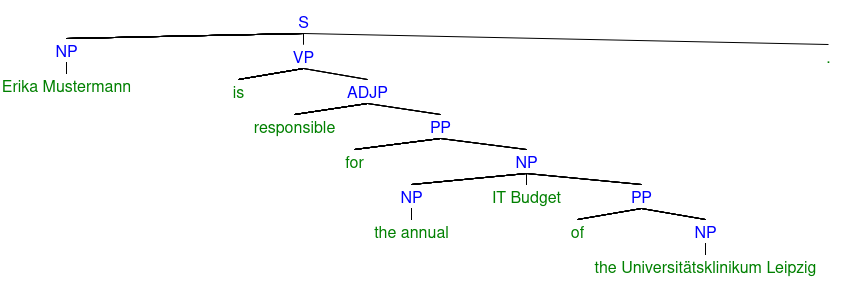
\includegraphics[width=\textwidth, height=\textheight, keepaspectratio]{Images/syntaxtree.png}
\caption[Beispielhafter Syntaxbaum]{Beispielhafter Syntaxbaum. Erstellt mit Link Grammar \citep{grammarparser} und \url{www.mshang.ca/syntree}.
\emph{S: Sentence; NP: noun phrase; VP: verb phrase; ADJP: adjective phrase; PP: prepositional phrase}.
Eingegebener Satz: \enquote{Erika Mustermann is responsible for the annual IT Budget of the Universitätsklinikum Leipzig.}}
\label{fig:syntaxtree}
\end{figure}
%Ein Satz wie \enquote{Das Kind rief seine Eltern mit seinem Rucksack.} kann entweder bedeuten, dass das Kind seine Eltern mithilfe seines Rucksacks ruft, oder dass die Eltern den Rucksack des Kindes haben.\todo{Beispiel aus Fachgebiet!}
%Es ist natürlich deutlich wahrscheinlicher, dass die Eltern des Kindes den Rucksack haben, was ein \ac{nlp}-Programm erkennen muss.
%Mit mehr Informationen könnte allerdings auch die andere Deutung möglich sein, ein \ac{nlp}-Programm steht stets in der Gefahr, voreilige Schlüsse zu ziehen.
%Desweiteren muss es analysieren, wer mit \enquote{sein} überhaupt gemeint ist.
%Dafür kann auch mehr Kontext nötig sein, welcher je nach Eingabe nicht immer vorhanden ist.

\subsection{NLP-Pipeline}
In einer Pipeline werden verschiedene Komponenenten eines Algorithmus oder Verfahren nacheinander ausgeführt.
Eine \ac{nlp}-Pipeline führt verschiedene Teilprogramme aus, da das Feld an sich zu komplex ist, als dass die Arbeit eines Programms es vollkommen lösen könnte.
Dabei gibt der Nutzer, hier ein Programmierer, der z.B. ein Question Answering-Programm schreiben will, der Pipeline die Daten, welche je nach Pipeline annotiert vorliegen müssen \citep{curatorpipeline}.
\ac{nlp}-Pipelines verwenden \acp{nn}, um funktionieren zu können.
Zwei Pipelines werden in \cref{ch:relatedWork} näher betrachtet.

\subsection{NLP-Modelle}

Modelle für \acl{nlp} verwenden heutzutage meistens Deep Learning.
Dazu werden sie vortrainiert, dass heißt sie werden schon vor der Anwendung mit einem Verzeichnis an Wörtern bzw. Sätzen,
wie zum Beispiel dem englischsprachigen Wikipedia mit etwa 2,5 Millionen Wörtern,
oder dem BooksCorpus \citep{bookscorpus},
einer Sammlung von Sätzen aus Büchern mit insgesamt etwa 800 Millionen Wörtern,
trainiert \citep{BERT}.
Mit \emph{fine-tuning-} oder \emph{feature-basiertem} Training\todo{fine-tuning- und feature-basiertes Training}
\todo{jetzige subsubsections evtl. in State of the Art umlegen?}

\subsubsection{ELMo}
\ac{elmo}
% feature-basiert
\todo{ELMo}

\subsubsection{BERT}
\ac{bert}
% finetuning-basiert
\todo{BERT}

\subsubsection{Andere Technologien}
\todo{Kurz andere Modelle erwähnen}

\section{Maschinelles Lernen und neuronale Netze}

Neuronale Netze sollen, indem sie die Struktur des menschlichen Gehirns nachstellen, komplexe Aufgaben, wie etwa das autonome Fahren oder \acl{nlp}, ausführen.
Dazu werden \emph{Knoten} oder \emph{Neuronen} in verschieden Schichten miteinander verbunden.
Es gibt drei Arten von diesen: Eingabe- (input), versteckte (hidden) und Ausgabe-Schichten (output).
Zwischen den Schichten sind die Knoten verbunden, jede Verbindung hat ein bestimmtes Gewicht, wie in \cref{fig:struktur-nn} dargestellt wird.
Mit diesem Gewicht wird der weitergereichte Wert multipliziert, welcher in der Eingabeschicht erstmals festgelegt wird.
Bei jedem Knoten werden die aus den niederen Schichten ankommenden Werte addiert, sodass ein neuer Wert entsteht.
Diese Summe wird dann mithilfe einer Funktion, meistens einer hyperbolischen oder Sigmoidfunktion ($sig(t)=\frac{1}{1+e^{t-1}}$), verändert und dann wieder weitergereicht.
Es werden genau diese Funktionen genommen, da deren Ableitungen die Fehlerberechnung leichter machen \citep{deeplearningnature}.
So kann das, je nach der Anzahl der versteckten Schichten, lange weitergehen.
Anfangs gab es meist nur eine versteckte Schicht, später wurden mehrere von diesen eingefügt und sogenannte \aclp{dnn} enstanden.
\begin{figure}%[htbp!]
\centering
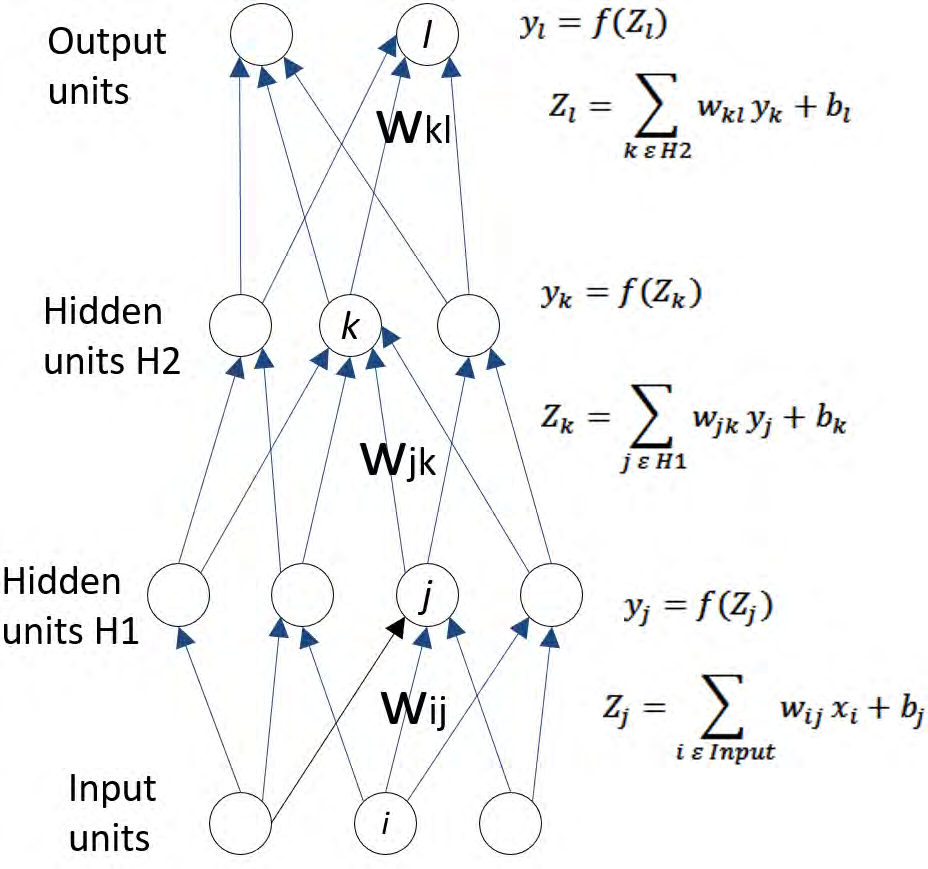
\includegraphics[width=.8\textwidth, height=.9\textheight, keepaspectratio]{Images/NeuralNetwork.png}
\caption[Struktur von DNNs]{Darstellung der Struktur eines mehrschichtigen neuronalen Netzes und der Fehlerberechnung. Quelle: \citet{deeplearningarchitecturesreview}}
\label{fig:struktur-nn}
\end{figure}

\subsection{Deep Learning}
Deep Learning ist ein Teilgebiet des maschinellen Lernens, das \acp{nn}, zu Deutsch \emph{neuronale Netze}, mit mehreren versteckte Schichten enthält \citep{deeplearningreview}.
Es befasst sich mit \acp{dnn}, welche häufig eine deutlich höhere Effizienz als \acp{nn} mit nur einer versteckten Schicht aufweisen.
Das bedeutet, dass die Ergebnisse für weniger oder gleich viel Training bessere Ergebnisse erzielen.
Die Qualität der Ergebnisse lässt sich z.B. bei der Klassifizierung von Bildern gut ermitteln.
Hier wird dem \ac{nn} ein Bild als Eingabe gegeben, welches es dann einordnen und beispielsweise die dargestellten Objekte, wie zum Beispiel Ampeln, erkennen soll.
Für Deep Learning gibt es verschiedene Architekturen.

\subsection{Convolutional Neural Network}
\acp{cnn} werden vor allem zur Bilderkennung und \ac{nlp} verwendet.
Sie sind auf dem visuellen Kortex des Menschen basiert, was sich in der dreidimensionalen Anordnung der Knoten verdeutlicht,
welche in \cref{fig:struktur-cnn} dargestellt ist.
Die Neuronen sind auf jeder Schicht, welche hier auch \emph{Filter} oder \emph{Kern} genannt werden,
zweidimensional aufgebaut, aber nicht wie sonst zu jedem Neuron der nächsten Schicht verbunden,
sondern nur zu einem \emph{lokalen rezeptiven Feld} \citep{deeplearningnature},
also einer kleineren Gruppe an Knoten, in der nächsten Schicht zusammengeschlossen.
Dies verkürzt die Trainingszeit, da jeder Knoten nur einen Teil der Eingabe sieht, aber alle nach dem gleichen Muster suchen.
Die kürzere Trainingszeit ist auch dadurch bedingt, dass manche Schichten ihre Gewichte teilen.
Für die eigentliche Klassifikation der Eingabe sind dann allerdings die hinteren Schichten vollständig verbunden.
\begin{figure}%[htbp!]
\centering
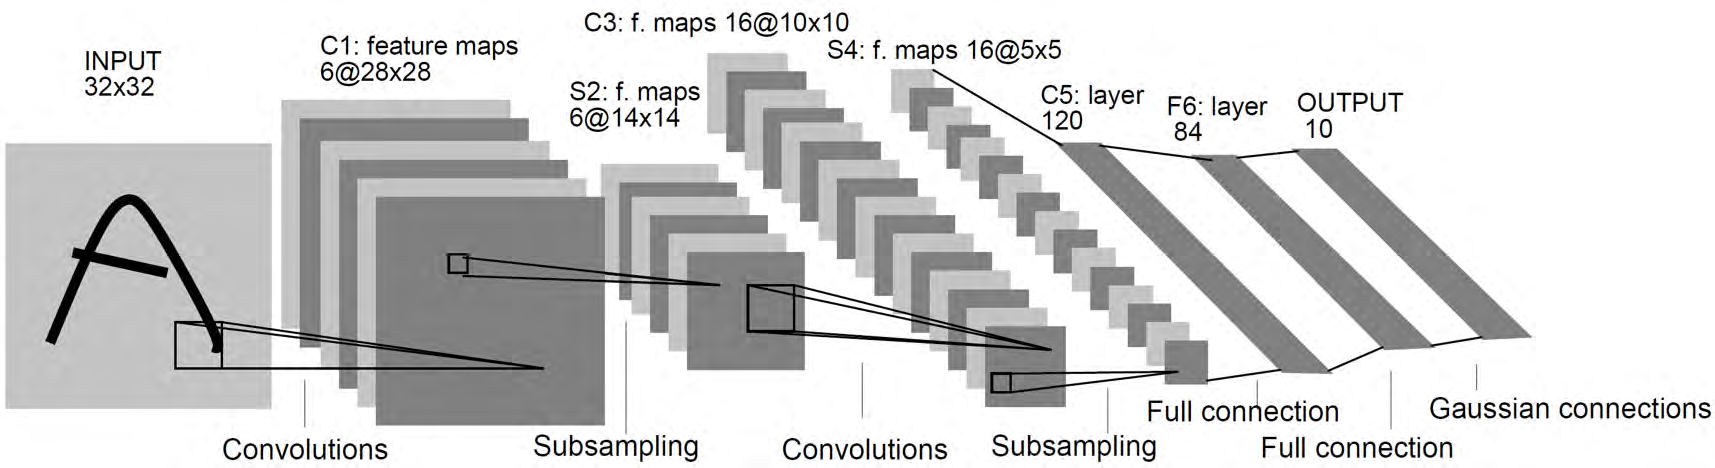
\includegraphics[width=\textwidth, height=\textheight, keepaspectratio]{Images/CNN.png}
\caption[Struktur von CNNs]{Die Struktur eines \ac{cnn} \citep{deeplearningarchitecturesreview}.}
\label{fig:struktur-cnn}
\end{figure}

\subsection{Recurrent Neural Network}
In einem \ac{rnn} formen die Knoten einen Kreis, sodass die Ausgabe der einen Schicht die Eingabe einer anderen wird,
wodurch dem \ac{nn} Informationen über die Ausgaben aus den vorherigen Schichten bekannt sind (siehe \cref{fig:struktur-rnn}).
Typischerweise gibt es in solchen \acp{nn} nur eine Schicht.
Ein Vorteil dieser Art von \acp{nn} ist, das sowohl eine Reihe an Eingaben als auch eine Reihe an Ausgaben möglich wird.
Dies ist besonders für Video- oder Audioverarbeitung äußerst praktisch \citep{deeplearningarchitecturesreview}.
\begin{figure}%[htbp!]
\centering
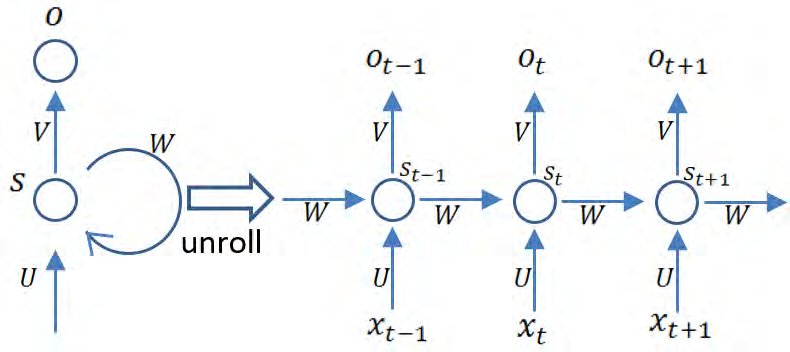
\includegraphics[width=\textwidth, height=\textheight, keepaspectratio]{Images/RNN.png}
\caption[Struktur von RNNs]{Die Struktur eines \ac{rnn} \citep{deeplearningarchitecturesreview}.}
\label{fig:struktur-rnn}
\end{figure}

\acp{rnn} werden außerdem für Encoder-Decoder-Modelle \citep{seq2seqB} verwendet.
Diese bestehen aus zwei \acp{rnn}, eines von ihnen ist ein Encoder (Verschlüsseler), das andere ein Decoder (Entschlüsseler
Besonders ist, dass die einzelnen \acp{nn} nicht einzeln, sondern das gesamte System zusammen trainiert wird \citep{seq2seqA}.
Sie wurden zuerst für maschinelle Übersetzung eingesetzt, sind jetzt aber als Methode etabliert.

Der sogenannte Attention-Mechanismus (Aufmerksamkeitsmechanismus) basiert auf dem Encoder-Decoder-Modell.
Es löst das Problem des Modells, dass dort alle Informationen der Eingabe in einen Vektor bestimmter Länge getan werden müssen
und somit Probleme bei langen Sätzen wie diesem hier entstehen könnten.
Der Attention-Mechanismus löst dieses Problem, indem bei jeder Iteration ein variabler Kontextvektor erzeugt wird \citep{attentionintro}.
Dieser ähnelt sehr der menschlichen Aufmerksamkeit, was den Namen des Mechanismus erklärt.
Für die \ac{rnn} werden statt \acsp{lstm} \acsp{gru} verwendet.

\subsection{Long short-term memory und Gated Research Units}
\ac{lstm}, zu Deutsch \enquote{langes Kurzzeitgedächtnis}, ist eine Form von \acp{rnn} \citep{lstm}.
Es wird zum Beispiel von Google und Amazon für deren Stimmenerkennungssoftware genutzt.
Im Gegensatz zu \acp{rnn} hat \ac{lstm} nicht das Problem, dass der Gradient langsam verringert wird,
indem es aus mehreren Zellen, durch die eingegeben, ausgegeben und vergessen werden kann.
\ac{gru} sind ein anderer Typ simpler \acp{rnn} und wurden von \citet{gru} entwickelt.

\subsection{Training von neuronalen Netzen}
Neuronale Netze basieren darauf, trainiert zu werden.
Bei diesem Training werden die Gewichte der einzelnen Verbindungen zufällig verändert, sodass am Ende selbst die programmierende Person nicht weiß, wie genau es funktioniert.
Es gibt viele Trainingstypen, aber es wird vor allem zwischen zwei unterschieden: \emph{überwachtes} (supervised) und \emph{unüberwachtes} (unsupervised) Lernen \citep{mllearning}.
Diese haben jeweils noch Untertypen, diese werden hier allerdings nicht weiter betrachtet.
Beim überwachten Lernen hat das Programm eine kurierte und annotierte Eingabe, das Programm erhält ein Paar aus Eingabe und erwarteter Ausgabe.
Um zum Beispiel Bücher digitalisieren zu können sind viele Trainingsdaten nötig.
Dafür hat die Carnegie Melon University in Pittsburgh reCAPTCHA entwickelt, welches in seiner ersten Version ein Wort zeigte, welches der Benutzer abschreiben sollte \citep{recaptchabooks}.
Google kaufte es, um damit Bücher und Hausnummern automatisch zu digitalisieren.
Die Möglichkeiten dieser Technologie erstrecken sich bis hin zum autonomen Fahren, wo zur Erkennung von Straßenschildern, Ampeln und anderen Verkehrsteilnehmern enorme Datenmengen benötigt werden.
Google hat die Eingaben, muss sich für die Ausgaben allerdings an seine Nutzer wenden \citep{recaptchaav}.
Ohne die Ausgaben hätte man nämlich unüberwachtes Lernen.
Dieses gibt dem zu trainierenden \ac{nn} keine Lösung vor und ist eher zur allgemeinen Mustererkennung gut.
Ein weiterer Trainingsansatz ist das \ac{zsl}.
Hier soll das Programm anhand einer Beschreibung von Objekten lernen, sie zu erkennen.
Der große Vorteil hieran ist, dass keine annotierten Daten benötigt werden, um auch seltene oder neue Vorkommnisse sicher erkennen zu können.
Im Gegensatz zum überwachten Lernen sind die Daten hier nicht gekennzeichnet, d.h. dem Programm wird nicht übermittelt, was in der Eingabe ist \citep{zsl}.

\subsection{Regelbasiertes System}
Vor neuronalen Netzen wurden vor allem die äußerst strikten regelbasierten Systeme zur Lösung von komplexen Problemen genutzt.
Sie bestehen aus einer Wissensbasis und einem Regelinterpreter.
Die Wissensbasis enthält Regeln, welche aus einer \emph{Atendenz} (Bedingung) und einer \emph{Konsequenz} (Resultat) bestehen, und Fakten.
Wenn die Bedingung einer Regel wahr wird, folgt das Resultat.
Regelbasierte Systeme ermöglichen ausführliche Begründungen, welche stark dem subjektiven menschlichen Denken ähneln.
Wissen lässt sich außerdem häufig leicht in einer solchen Regelform ausdrücken.
Es gelten nicht immer alle Regeln und Fakten, sie können dynamisch ein- und ausgeschaltet werden \citep{rulebasedsystem}.
Regelbasierte Systeme werden heute weniger benutzt, in Verbindung mit neuronalen Netzen können sie jedoch immer noch sehr nützlich sein.
